\section{Implementation Details}
\label{sec:implement}

\begin{figure}[htbp]
\centering
\label{fig:fsinfs}
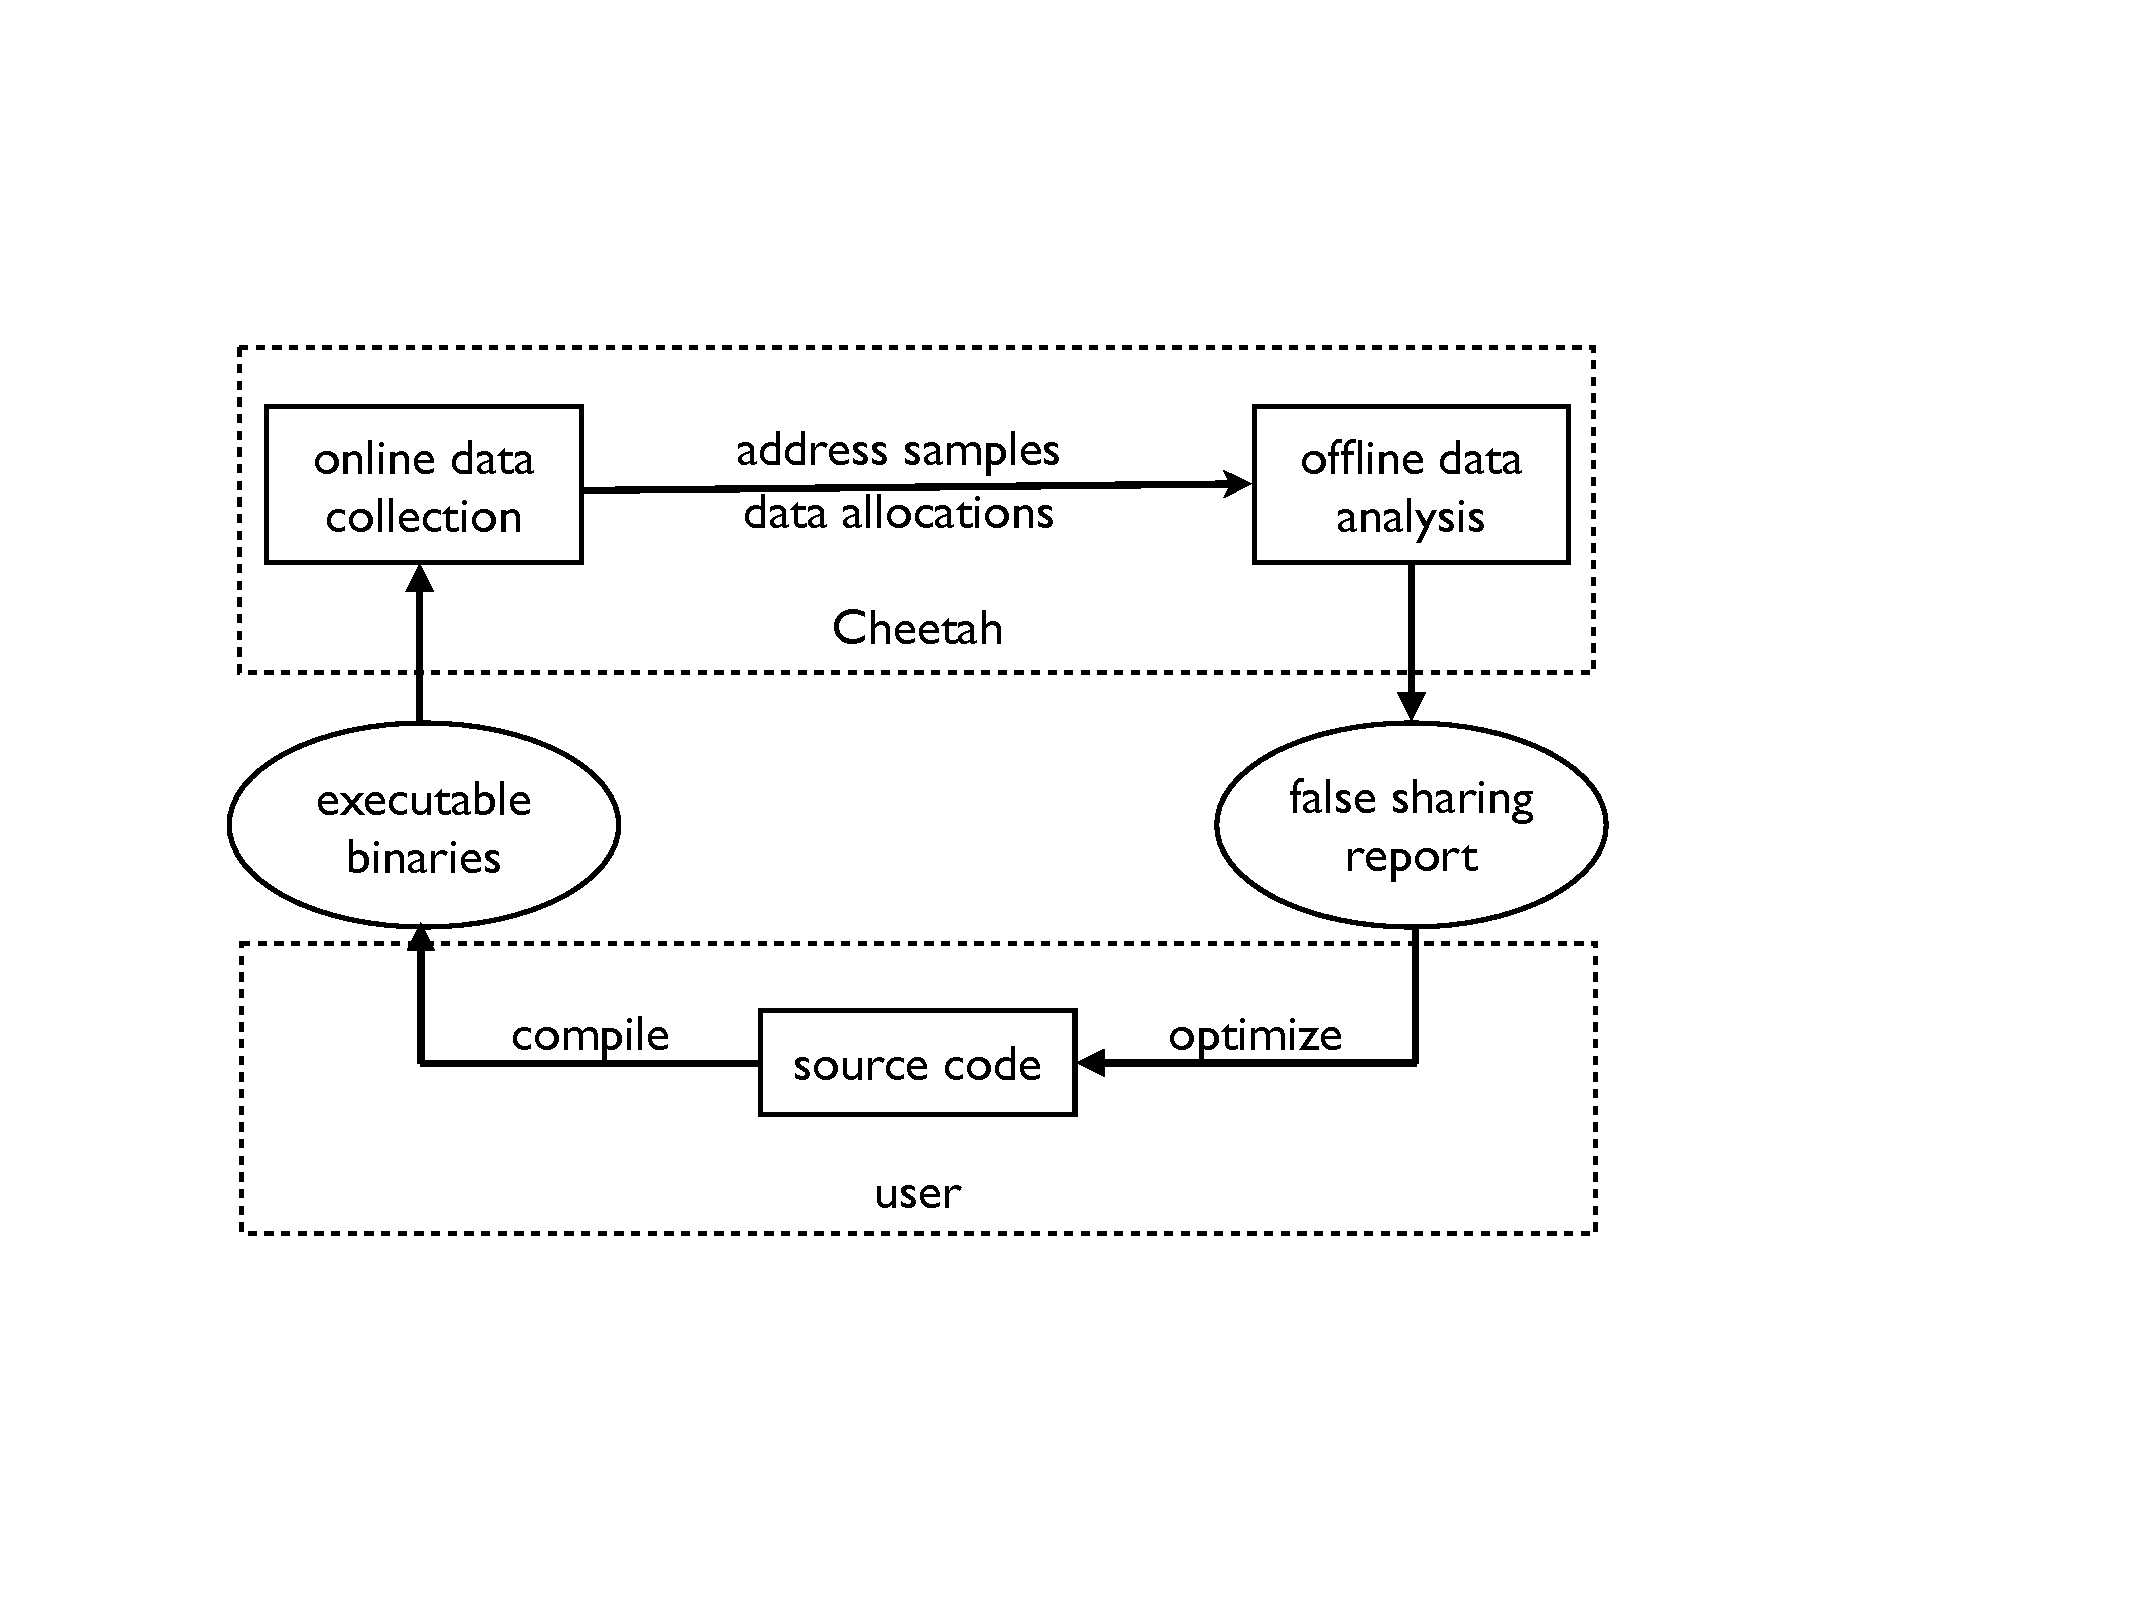
\includegraphics[width=\columnwidth]{figure/workflow}
\caption{The workflow of \cheetah{}}
\end{figure}

In this section, we describe the implementation of \cheetah{} and highlight our solutions in addressing technical challenges. Figure~\ref{} shows the workflow of \cheetah{}, 
which consists of an online and offline components. We elaborate these components in the rest of this section.

\subsection{Online Component}
The online component of \cheetah{} intercepts each thread by overloading the thread creation function, i.e., {\tt pthread\_create}. At meanwhile, \cheetah{} sets up the PMU for address sampling to let each thread accept samples individually. {\color{red} did you associate samples with data objects online? Is there any challenge in efficiently handling parallelism?}



\subsection{Offline Component}
{\color{red} How to merge all of the analysis results from different threads? What if there are many threads? How is the scalability of the analysis? What's the output? You can have a forward pointer to Section 6.}

%However, it is straightforward to solve such false sharing problems by using an allocator like Hoard that avoids this kind of false sharing.


%\subsection{Predicting False Sharing}
% What is the basic idea to predict false sharing problem?
% What is the difference with Predator{}?
% For those predicted false sharing, we cannot predict performance improvement?



 